\documentclass[a4paper,12pt]{report}
\usepackage{amsmath,amsfonts,amssymb,enumerate,graphicx,fancyhdr,times}
\usepackage{tabularx,float,xspace,float,caption,setspace,hyperref}
\usepackage[top=1in, left = 1in, right = 1in, bottom = 1in]{geometry}
\usepackage[utf8]{inputenc}

\pagestyle{fancyplain}
\fancyhf{}
\renewcommand{\headrulewidth}{0px}
\fancyfoot[R]{\thepage}
\parindent 0px

\begin{document}
\begin{titlepage}
	\begin{minipage}[t][3cm][b]{.2\linewidth}
		
\includegraphics[width=2.5cm, keepaspectratio]{cuet.png} \par \vspace{0.5cm}
	\end{minipage}
	\begin{minipage}[t][4cm][t]{.75\linewidth}
		\raggedleft
		\vspace{0.1cm}
		{\bfseries \Large CHITTAGONG UNIVERSITY OF ENGINEERING \& TECHNOLOGY}
		\par
		\vspace{.5cm}
		{DEPARTMENT OF COMPUTER SCIENCE AND ENGINEERING}
	\end{minipage}

	\centering

	\vspace{1cm}

	\raisebox{-\baselineskip}{\rule{\textwidth}{1px}}

	\rule{\textwidth}{1px}

	\vspace{0.2cm}
	{\large{{REPORT TITLE}}}\par \vspace{0.3cm}
	\Large{{Project proposal on \bfseries{E-code Analyzer}}}
	\rule{\textwidth}{2px}

	\vspace{0.5cm}

	\normalsize
	\begin{tabular}{cl}
		COURSE CODE        & : CSE 356                          \\
		COURSE NAME        & : SOFTWARE ENGINEERING (SESSIONAL) \\
		EXPERIMENT NO      & : 01                               \\
		DATE OF SUBMISSION & : 21 -- 11 -- 2023                 \\
	\end{tabular}

	\vspace{2cm}
	\begin{center}
		
\includegraphics[width=4cm, keepaspectratio]{remarks.png}
		\captionof*{figure}{REMARKS}
	\end{center}
	\parbox[l]{.5\linewidth}{\begin{center}
			Submitted By
		\end{center}
		\raggedright
		\begin{tabular}{ll}
			MD AKIB HASAN        & 1904015 \\[.1cm]
			K.M. MAHABUB HOSSAIN & 1904017 \\[.1cm]
			SADMAN RAHMAN ANANTA & 1904020 \\
		\end{tabular}
	}
	\parbox[r]{7.8cm}{\vspace{1.5cm}
	\begin{center}
		Supervised By
	\end{center}
	\raggedleft
	Annesha Das\\
	{\footnotesize
	Assistant Professor \\
	Department of CSE, CUET}\\[0.5cm]

	Sabiha Anan\\
	{\footnotesize
	Assistant Professor \\
	Department of CSE, CUET}

	}

	\vfill
\end{titlepage}


\onehalfspacing

\section*{Introduction}
E-numbers, short for Europe numbers, are codes assigned to substances used as food additives initially within the European Union (EU) and European Free Trade Association(EFTA). It is sometimes informally used as a term to refer to artificial food additives. The numbering scheme follows that of the International Numbering System (INS) as determined by the Codex Alimentarius committee.
\begin{figure}[H]
	\centering
	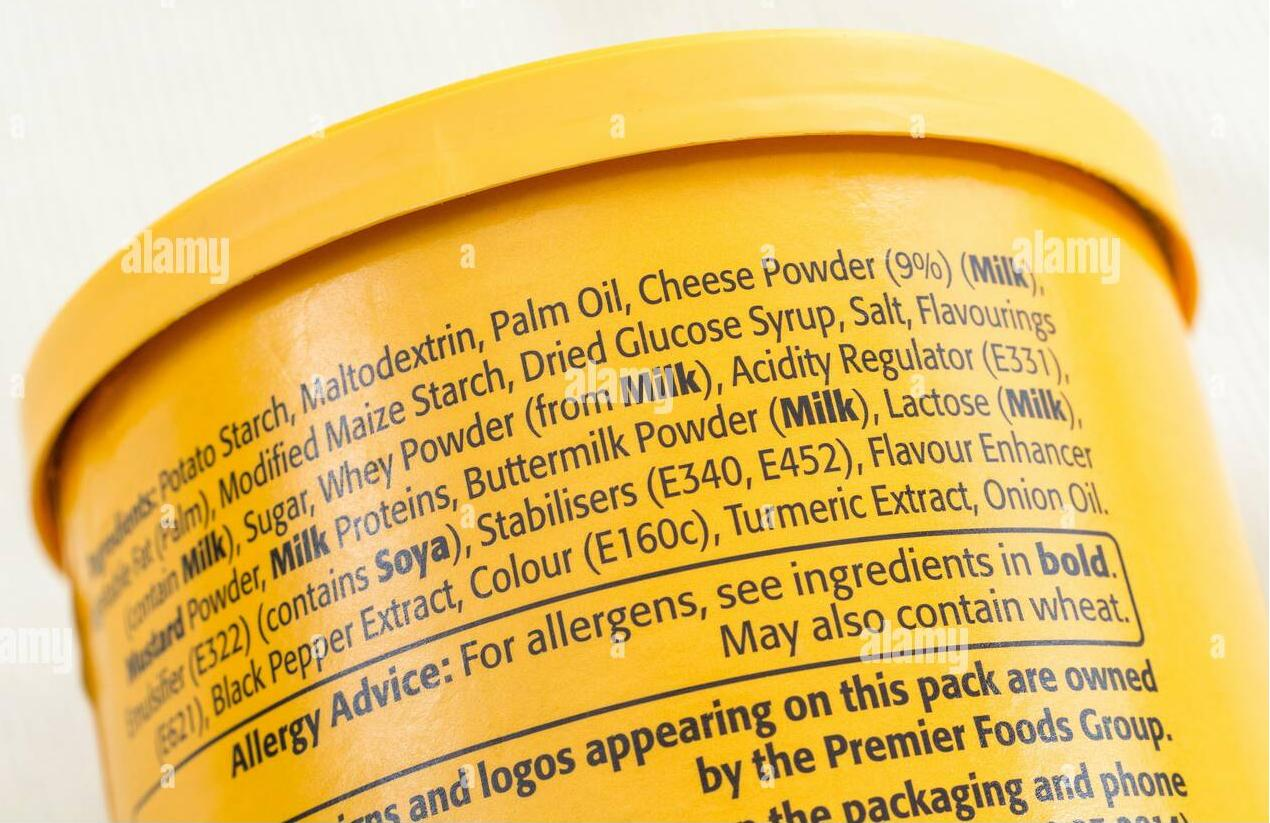
\includegraphics[width=8cm,keepaspectratio]{e-no2.jpg}
	\caption{E numbers}
\end{figure}
Each E-number corresponds to a specific food additive and is used as a labeling system on food products to inform consumers about the presence of these additives. The European Food Safety Authority (EFSA) evaluates and approves these additives based on scientific assessments of their safety for human consumption.



\section*{Scope}
\subsection*{Background}
Codes are used on food labels to indicate the presence of specific additives, which can include substances found naturally in foods such as vitamin C (E300), vitamin B2 (E101) or artificial additives avoparcin (E715) which is currently banned in EU.

It's worth noting that not all countries use the E-number system, and different countries may have their own systems for regulating and labeling food additives. In the United States, for example, the Food and Drug Administration (FDA) uses a different system, where food additives are often listed by their common names on ingredient labels.

\subsection*{Motivation}
Packaged products are one of the integral part of our daily life. Being more educated and conscious about health, religion etc. we are often interested in knowing what substances are present in our food. Due to growth and establishment of science and chemistry artificial substances has become popular among business products and that's why the idea of crosschecking of those gained importance recently in Muslims, vegetarians etc. communities.

Such as Muslims are not allowed to eat pork meat or anything comes from it \cite{muslim_pork_avoid} or vegans avoid any living animal produced products etc. There are some substances that can be harmful in various conditions as well as allergies in human body.
\begin{figure}[H]
	\centering
	\parbox{7cm}{
		
\includegraphics[width=5cm,keepaspectratio]{pork_haram.png}
	}
	\parbox{7cm}{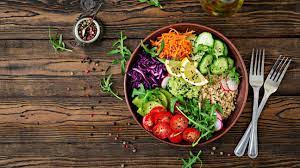
\includegraphics[width=5cm,keepaspectratio]{vegitables.png}}
	\caption{Different Customs and Beliefs}
\end{figure}
Therefore we expect a platform within our reach frequently with many features such as--
\begin{itemize}
	\item Determining Halal, Haram substances in packaged products.
	\item Differentiate between food and other products for vegans and vegetarians.
	\item Easy identification of the presence of harmful substances and additives in packaged food.
	\item Providing valid references and information sources for various qualities of artificial substances and additives.
\end{itemize}

\subsection*{Application}
An E-number platform could have several applications, particularly in the areas of health, religious and dietary practices. Some potential applications are enlisted below:
\begin{description}
	\item [Ingredient Awareness]: The app can help users identify and understand the E-numbers present in food products. This information can be valuable for individuals with food sensitivities or allergies.
	\item [Nutritional Information:] Provide nutritional information associated with each E-number, helping users make informed choices based on their dietary preferences and health goals.
	\item[Allergen Alert:] The app can alert users to the presence of specific E-numbers associated with common allergens, facilitating safe food choices for individuals with allergies.
	\item[Vegan and Vegetarian Diets:] Help users following vegetarian or vegan diets identify E-numbers that may be derived from animal products.
	\item[Halal and Kosher Compliance:] The app can assist users in adhering to Halal or Kosher dietary laws by identifying E-numbers that may be derived from non-permissible sources.
	\item[Religious Fast Observance:] During periods of religious fasting, the app could help users find food products that comply with fasting restrictions by avoiding certain E-numbers.
	\item[Label Translation:] For individuals who may not understand the language on food labels, the app can translate and explain E-numbers, promoting ingredient transparency.
	\item[Educational Resource:] Serve as an educational tool, providing users with information on the purpose and safety of different E-numbers.
	\item[Environmental Impact:]
		The app can include information on the environmental impact of certain E-numbers, promoting awareness and encouraging users to make sustainable food choices.
	\item[	Children's and Expectant Mothers' Health:] Parents can use the app to make informed choices about the food products they give to their children, considering any potential health effects of E-numbers.

\end{description}
\section*{Related works}
There are several apps and websites with some limited accessibility and features on e number and its acceptability in various aspect. Such as --
\begin{itemize}
	\item EU parliament provides valid substances in 2008. \cite{eu_perlament}
	\item New Zealand based skin related websites provides some descriptive information about those additives. \cite{dermnet_nz}
	\item International Halal Certification(IHC) from Pakistan provides Halal Certification body in their website. \cite{pak}
	\item The Wikipedia page of E number has the latest references. \cite{wiki_enumber}
	\item The Vegetarian Society from UK has a list of codes that should or shouldn't be taken as a vegetarian. \cite{veggie}
	\item An android provides Halal codes where the source of information is not included. \cite{halal_app}
\end{itemize}
Moreover there are \emph{E-code verifier}\cite{ecodeverifier}, An-Najah National University publication \cite{palestine} and data from IRC \cite{halal_singapore} by Govt. of Singapore are worth mentioning.
\begin{figure}[H]
	\centering
	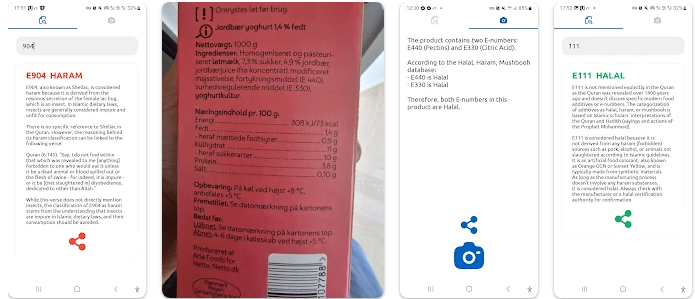
\includegraphics[width=12cm,keepaspectratio]{halal_app.png}
	\caption{"Halal Check E-number \& E-codes" App}
\end{figure}
\subsection*{Drawbacks}
There are different sources, and it's very difficult to search for specific codes while having snacks in hand before eating. Because these sources are published in different ways and in different websites. Moreover, the \emph{E-code verifier} app available only in android platform not iOS and Windows or Linux etc. It also provides only halal-haram information, but the source is not clear. Therefore, our proposed application is expected to overcome these drawbacks.

\subsection*{Proposed Improvements}
Our goal is to overcome the drawbacks of current sources and make data more human-readable and efficient. We intend to combine features such as --
\begin{itemize}
	\item Barcode reader,
	\item Personalized information,
	\item Fast search using E-number/substances names,
	\item Valid data sources etc.
\end{itemize}

\section*{Process Description}
This platform is expected to help people navigate the world of E-numbers, providing valuable information on food additives while considering their unique health, allergy, and religious preferences.

\subsection*{Key Features:}
\begin{enumerate}
	\item {\bfseries E-Number Lookup:}
	      \begin{itemize}
		      \item Quickly search and identify E-numbers on food labels.
		      \item Access detailed information about each additive, including its purpose and potential health effects.
	      \end{itemize}
	\item {\bfseries Personalized Profiles:}
	      \begin{itemize}
		      \item Create a personal profile with login credentials for a customized experience.
		      \item Input health conditions, allergies, and religious preferences to tailor the app to your specific needs.
	      \end{itemize}
	\item {\bfseries Allergy Alerts:}
	      \begin{itemize}
		      \item Provide instant alerts when a product contains an E-number associated with your specified allergies.
		      \item Being confident in food choices, whether anyone has gluten, dairy, nut, or other allergies.
	      \end{itemize}
	\item {\bfseries Religious Preferences:}
	      \begin{itemize}
		      \item Setting religious preferences to filter out E-numbers that may not align with the dietary restrictions.
		      \item Ideal for those adhering to Halal, Kosher, or other religious dietary guidelines.
	      \end{itemize}
	\item {\bfseries Nutritional Information:}
	      \begin{itemize}
		      \item Access nutritional details for each E-number to make informed decisions about your diet.
		      \item Keeping track of calorie counts, macronutrients, and other essential information that can be manipulated by the additives.
	      \end{itemize}
	\item {\bfseries Barcode Scanner:}
	      \begin{itemize}
		      \item Using barcode scanner to quickly analyze products while shopping.
		      \item Instantly see if a product contains E-numbers that match your personalized criteria.
	      \end{itemize}
	\item {\bfseries Data Sources}
	      \begin{itemize}
		      \item Provide multiple Accurate data sources for every information about E-numbers or concerned additives.
		      \item Thoughts and preferences form scientists and scholars from respective fields are crucial.
	      \end{itemize}
\end{enumerate}

\section*{Development Tools}
There are various tools we are expecting to use in this project. Such as--
\begin{itemize}
	\item Flutter
	\item Firebase
	\item Flutter gallery, driver, flutterflow, canva
	\item Google play etc.
\end{itemize}
\section*{Conclusion}
Health awareness is one of the important aspect with the development of modern civilization with science and technology. With various artificial additives to improve the taste and quality of food, there are religious and other social obligation we need to embrace. A well documented and user satisfactory platform with solid information sources can play a vital role in healthy life and our future.

\renewcommand{\bibname}{\Large Bibliography}
\bibliographystyle{ieeetr}
\bibliography{reference}

\end{document}
